% secciones/resultados.tex -- Sec 3 Resultados

\subsection{Verificación de la implementación}
\label{sec:verificacion}

Antes de la calibración, la implementación del núcleo larvario se verificó contra el archivo de modelación publicado por \textcite{eriksenDynamicModellingFeed2022} como material suplementario, con comparación fórmula a fórmula; las dos divergencias encontradas entre sus ecuaciones impresas y su propio archivo ---y la decisión de replicar el archivo--- se documentan en el Material Suplementario (sec.~\ref{sup:correspondencia}). Esta verificación garantiza que el código implementa el modelo de referencia tal como su autor lo opera numéricamente; su transferibilidad al sistema experimental de este estudio es, precisamente, lo que las secciones siguientes evalúan.

\subsection{Ajuste de calibración}
\label{sec:ajuste}

La calibración completa (tres etapas, sec.~\ref{sec:calibracion}) reduce el RMSE censurado conjunto de los ocho cierres de 180.53~ppm/min con el modelo de referencia sin ajustar (E0) a 86.41~ppm/min con el modelo completo (C) ---una reducción del 52.1~\%---; el RMSE crudo es 94.67~ppm/min. En el bloque de crecimiento, el RMSE de la fase de ajuste (días $\le 8$) es 36.2~mg de peso fresco por larva. El Cuadro~\ref{tab:cierres} compara las observaciones con las predicciones de C punto a punto; el Cuadro~\ref{tab:calibrados} reporta los parámetros estimados, con los que alcanzaron una frontera de su intervalo marcados como tales, en la convención del estudio. La Figura~\ref{fig:propios} muestra las trayectorias completas y la descomposición de C en sus componentes larvario y microbiano: el aporte microbiano crece a lo largo del ciclo pero permanece acotado por el pastoreo, mientras la larva domina la fase central.

\begin{table}[htbp]
  \centering
  \caption{Cierres de gas del experimento propio y predicciones del modelo completo (C, con módulo de prepupa). Los valores precedidos de $\ge$ son cotas inferiores: el cierre saturó el sensor.}
  \label{tab:cierres}
  \begin{tabular}{llrrl}
    \toprule
    Dieta & Día & Observado (ppm/min) & Modelo C & Saturado \\
    \midrule
    D1 & 6  & $\ge 670.56$ & 459.85 & sí \\
    D1 & 6  & $\ge 474.23$ & 459.85 & sí \\
    D1 & 8  & $\ge 311.82$ & 421.25 & sí \\
    D1 & 10 & 285.57       & 304.14 & no \\
    D4 & 6  & 228.52       & 301.49 & no \\
    D4 & 8  & $\ge 383.67$ & 356.65 & sí \\
    D4 & 10 & 104.11       & 155.85 & no \\
    D4 & 14 & 79.11        & 156.84 & no \\
    \bottomrule
  \end{tabular}
\end{table}

\begin{table}[htbp]
  \centering
  \caption{Parámetros calibrados del modelo. Los marcados con frontera alcanzaron el límite de su intervalo de búsqueda y se reportan como tales.}
  \label{tab:calibrados}
  \begin{tabular}{llll}
    \toprule
    Etapa & Parámetro & Valor & Frontera \\
    \midrule
    1 & $k_{\mathrm{ref}}$ (D1 / D4) & 1.0 / 1.0~d$^{-1}$ & superior (ambas) \\
    1 & $\delta_{CS}$ (D1 / D4) & 0.950 / 0.798 & superior (D1) \\
    2 & $a_{\max}$ & 1.4999~d$^{-1}$ & superior \\
    2 & $\rho$ & 9.640~mg~C~d$^{-1}$ & no \\
    2 & $f_{D4}$ & 0.7172 & no \\
    2 & $\gamma$ & 0.5798 & no \\
    3 & $f_{\mathrm{mant}}$ & 0.05 & inferior \\
    3 & $k_{\mathrm{cat}}$ & 0.1264~d$^{-1}$ & no \\
    \bottomrule
  \end{tabular}
\end{table}

\begin{figure}[htbp]
  \centering
  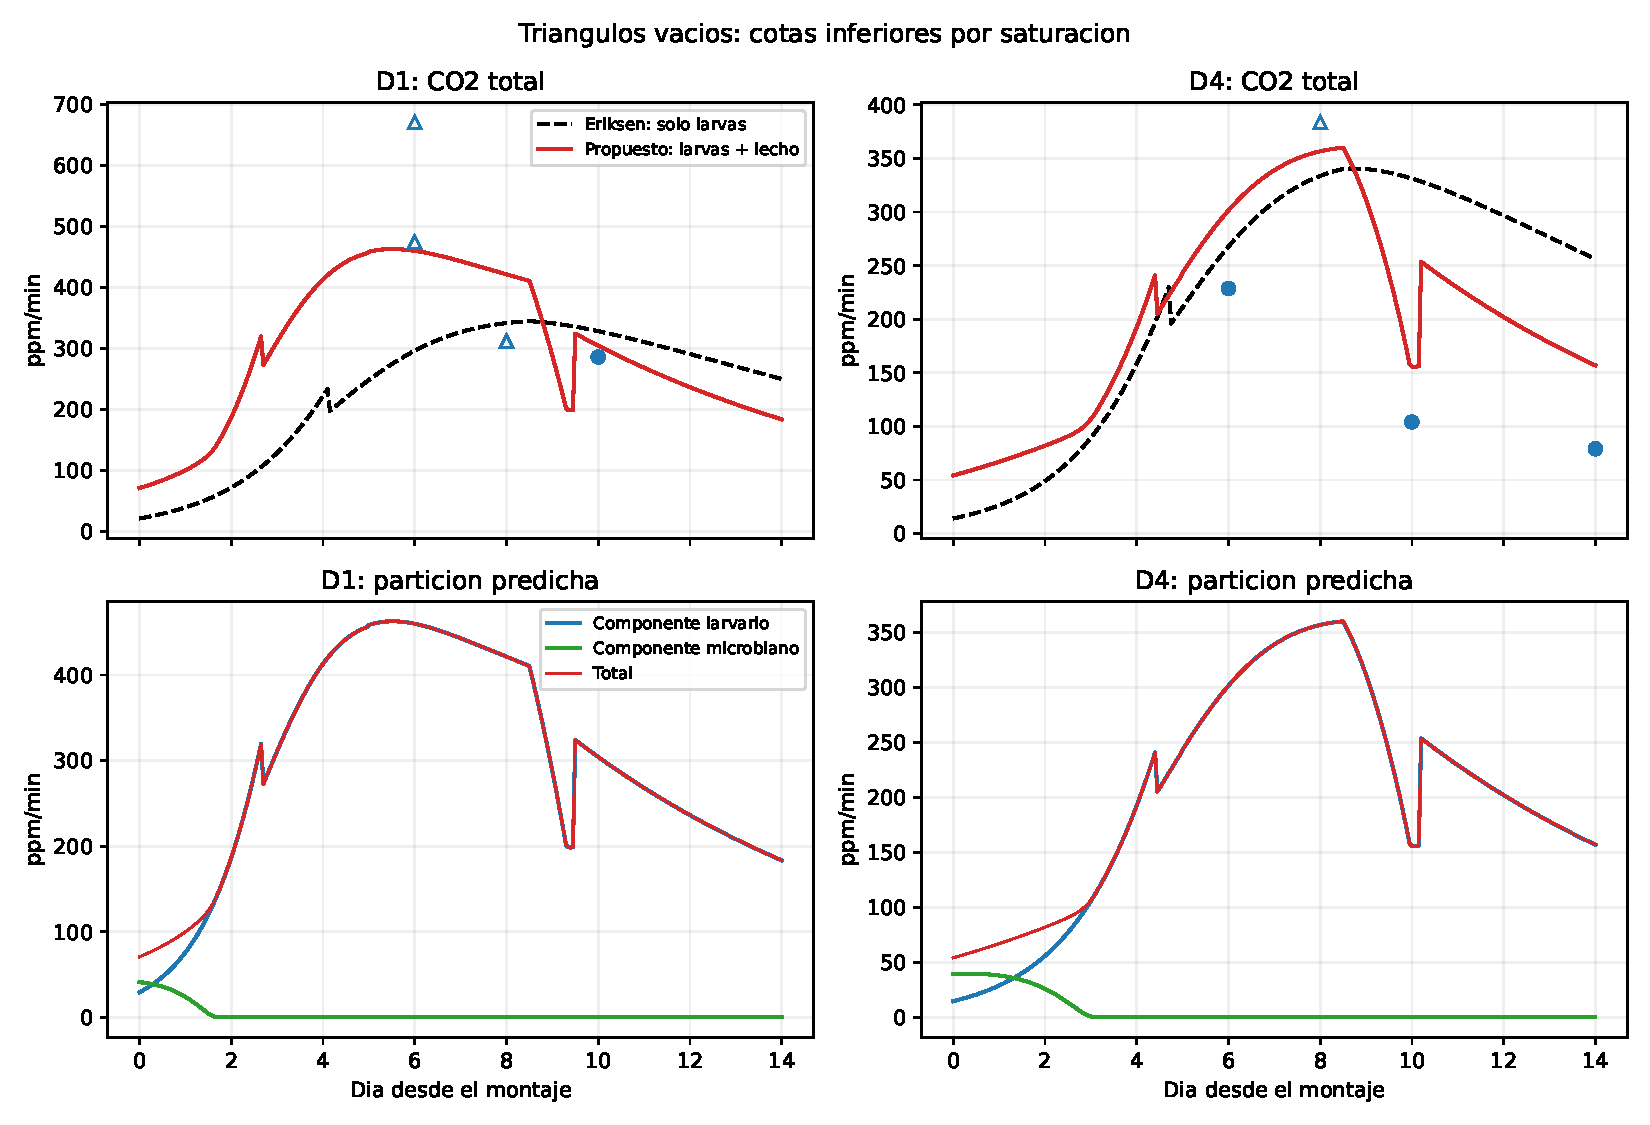
\includegraphics[width=\textwidth]{figuras/datos_propios_modelos.pdf}
  \caption{Datos propios. Paneles superiores: modelo de referencia sin ajustar (E0) y modelo completo (C) frente a los cierres observados. Paneles inferiores: descomposición de C en sus componentes larvario y microbiano. Los triángulos vacíos son cotas inferiores por saturación del sensor.}
  \label{fig:propios}
\end{figure}

\subsection{Atribución y capacidad predictiva fuera de muestra}
\label{sec:atribucion}

La comparación anidada de las cuatro configuraciones (sec.~\ref{sec:calibracion}) se evaluó con validación cruzada interna agrupada por dieta y día: en cada uno de los siete pliegues se recalibraron las etapas con los días restantes y se predijo el día excluido, de modo que cada cierre de tratamiento fue predicho una única vez fuera de la calibración. El Cuadro~\ref{tab:cv} resume los resultados.

El modelo completo (C) es el mejor fuera de muestra: su RMSE censurado, 130.97~ppm/min, reduce el del modelo de referencia (E0, 180.53) en un 27.4~\%, y en los cuatro cierres no saturados la reducción es del 14.3~\% (125.74 frente a 146.81~ppm/min). La recalibración del núcleo sola (R) mejora modestamente (164.41, $-8.9$~\% frente a E0). En cambio, añadir el lecho con el núcleo original pero sin acople ni pastoreo (A) degrada la predicción por encima de la línea base (575.47~ppm/min): la dinámica microbiana sin control top-down sobre-emite en la fase tardía. Este contraste cuantifica la conclusión mecanística: el lecho solo es útil cuando la larva lo controla. Los parámetros de C son estables entre pliegues ($a_{\max}$ entre 1.47 y 1.50; $\gamma$ entre 0.48 y 0.69), lo que indica que el ajuste no depende de un día particular.

\begin{table}[htbp]
  \centering
  \caption{Validación cruzada interna (siete pliegues por dieta y día): RMSE fuera de calibración y cobertura de las cotas saturadas, conjunto de las dos dietas. Los valores exactos usan solo los cuatro cierres no saturados.}
  \label{tab:cv}
  \begin{tabular}{lrrl}
    \toprule
    Configuración & RMSE censurado (ppm/min) & RMSE exactos (ppm/min) & Cobertura saturados \\
    \midrule
    E0 (referencia) & 180.53 & 146.81 & 1/4 \\
    R (recalibrado) & 164.41 & 160.63 & 2/4 \\
    A (lecho, núcleo original) & 575.47 & 808.89 & 3/4 \\
    C (completo) & 130.97 & 125.74 & 1/4 \\
    \bottomrule
  \end{tabular}
\end{table}

\subsection{Incertidumbre de la mejora}
\label{sec:bootstrap}

La incertidumbre de la mejora se estimó remuestreando 5000 veces las predicciones fuera de calibración, con remuestreo agrupado por dieta y día. Para C, la reducción del RMSE censurado frente a E0 tiene mediana $+27.7$~\%, intervalo percentil $(-42.8, +46.0)$, y es positiva en el 90.9~\% de los remuestreos; el RMSE censurado de C tiene mediana 130.97~ppm/min y percentiles (64.5, 168.9). Estos intervalos describen el remuestreo de siete días de medición, no una validación independiente, y la fracción de mejora positiva no constituye una probabilidad de superioridad; se reportan como medida exploratoria de la estabilidad del resultado.

\subsection{Límites declarados}
\label{sec:limites}

Tres límites se declaran junto con los resultados. Primero, la cobertura de las cotas saturadas es de 1/4 (Cuadro~\ref{tab:cv}): en tres de los cuatro cierres saturados el modelo predice por debajo de la cota observada, de modo que la reducción del RMSE censurado no implica que todas las predicciones superen los límites instrumentales. Segundo, la fase tardía no entró al ajuste de las etapas 1 y 2 (opción declarada en sec.~\ref{sec:calibracion}): en los días 10 y 14 el modelo sobre-predice el peso de las larvas (residuos de $+113$, $+46$, $+63$ y $+14$~mg en D1-10, D1-14, D4-10 y D4-14), consistente con el vaciado intestinal de la prepupa, que el módulo de la etapa 3 reduce pero no elimina. Tercero, cuatro parámetros alcanzaron una frontera de su intervalo de búsqueda (Cuadro~\ref{tab:calibrados}) y se reportan como límites del ajuste, no como estimaciones puntuales precisas.
